\section*{Introduction}

This report explains the implementation details of CS523 Computer Vision
Assignment 3, which is about classifying a 4-class dataset with bag of features.
The general idea behind a bag of visual words is to represent an image as a set
of features. Features consist of keypoints and descriptors and no matter if an
image is rotated, shrinked or expanded, the keypoints will always be the same. A
descriptor is the description of a keypoint. The keypoints and descriptors are
used to construct vocabularies and represent each image as a frequency histogram
of features that are in the image. By using the frequency histogram, we can
find and predict the category of an image.

\section*{Running the code}
To run the code, you need to re-organize the dataset to look something similar
to:

\dirtree{%
    .1 dataset.
    .2 train.
    .3 airplanes.
    .3 cars.
    .3 faces.
    .3 motorbikes.
    .2 test.
    .3 airplanes.
    .3 cars.
    .3 faces.
    .3 motorbikes.
}

After modifying the directory structure, you should call main.py with the
parameters that are needed to run the experiment you want. For example, the
following snippet will set the feature extraction method to keypoints, will use
kmeans, k=50 for the clustering algorithm.

python main.py --train\_path dataset-modified/train --test\_path
dataset-modified/test --no\_clusters 50 --clustering\_alg kmeans --feature\_extraction kp



\section*{Feature Extraction and Description}



%Principal Component Analysis(PCA) is an algorithm used for dimensionality
%reduction. In the MNIST hand written digits dataset, each image comes as vectors
%of dimension 784. However, we do not need all the dimensions contain classifying
%an image.  The idea is, compressing a matrix with a lot of features into a
%smaller matrix, with less features which preserves as much of the information in
%the full matrix as possible.

%In my PCA algorithm, to get the eigen vectors, I first calculated the mean
%values of each column and centered the values I found by subtracting the mean
%column value. Afterwards, I calculated the covariance matrix of the centered
%matrix. Than, I calculated the eigen values and eigen vectors with and than
%finally, sorted them with respect to their eigen value magnitudes.

%To get the reduced versions of the images, I projected both train images and
%test images on their first 25 principal components by a matrix multiplication.
%To visualize the results, I used a function I found online to reconstruct the
%first image of the MNIST dataset from its principal components and ended up with
%the following image.

%\begin{figure}[H] \centering
%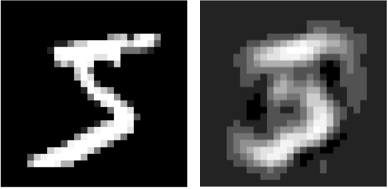
\includegraphics[width=\textwidth]{images/before-after-pca.png}
%\caption*{PCA results} \setlength{\belowcaptionskip}{-40pt}
%\setlength{\abovecaptionskip}{-40pt}
%\end{figure}

%To observe the clustering, I projected the train images onto their first two
%principal components and produced a scatter plot. 

%\begin{figure}[H]
%\centering
%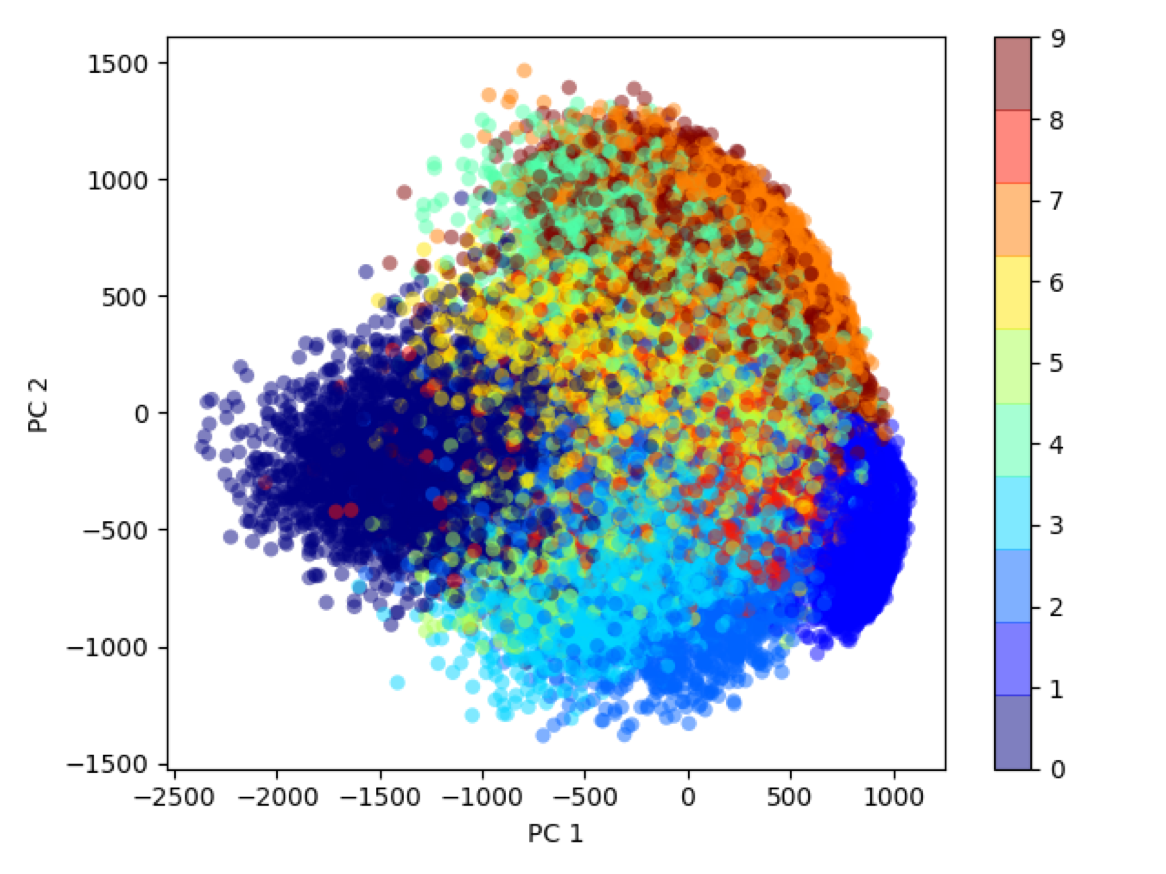
\includegraphics[width=\textwidth]{images/pca.png}
%\caption*{PCA results}
%\setlength{\belowcaptionskip}{-40pt}
%\setlength{\abovecaptionskip}{-40pt}
%\end{figure}



%k-Nearest Neighbors is a simple classification algorithm that stores all
%available cases and classifies new cases based on a similarity measure.

%After reducing the dimensions from 784 to 25, I computed the distances between
%X\_test and X\_train to prepare my data for kNN classifier. To compute the
%distances, I first used a nested for loop but ended up waiting 30 minutes for
%computing the distances between train data and test data. To compute the
%distances without any loops, I converted my nested for loops to a matrix
%multiplication with two broadcast sums.

%\begin{lstlisting}[language=Python, caption=Computing the distances without
%loops]
%dists = np.reshape(np.sum(X**2, axis=1), [num_test,1]) + np.sum(X_train**2, axis=1) \
%- 2 * np.matmul(X, X_train.T)
%dists = np.sqrt(dists)

%\end{lstlisting}

%After computing the distances and obtaining a distance matrix, I looped over the
%test data and used the distance matrix to find k nearest neighbors of the ith
%testing point. Than I used the train labels to find the neighbors of the found
%labels and than obtained the most common labels.

%To find the best k value for the classification of the MNIST dataset, I looped
%over k values from 0 to 15 and plotted the following graph to visualize my
%findings. Lastly, I calculated the confusion matrix for 6 neighbors.

%\begin{figure}[H]
%\centering
%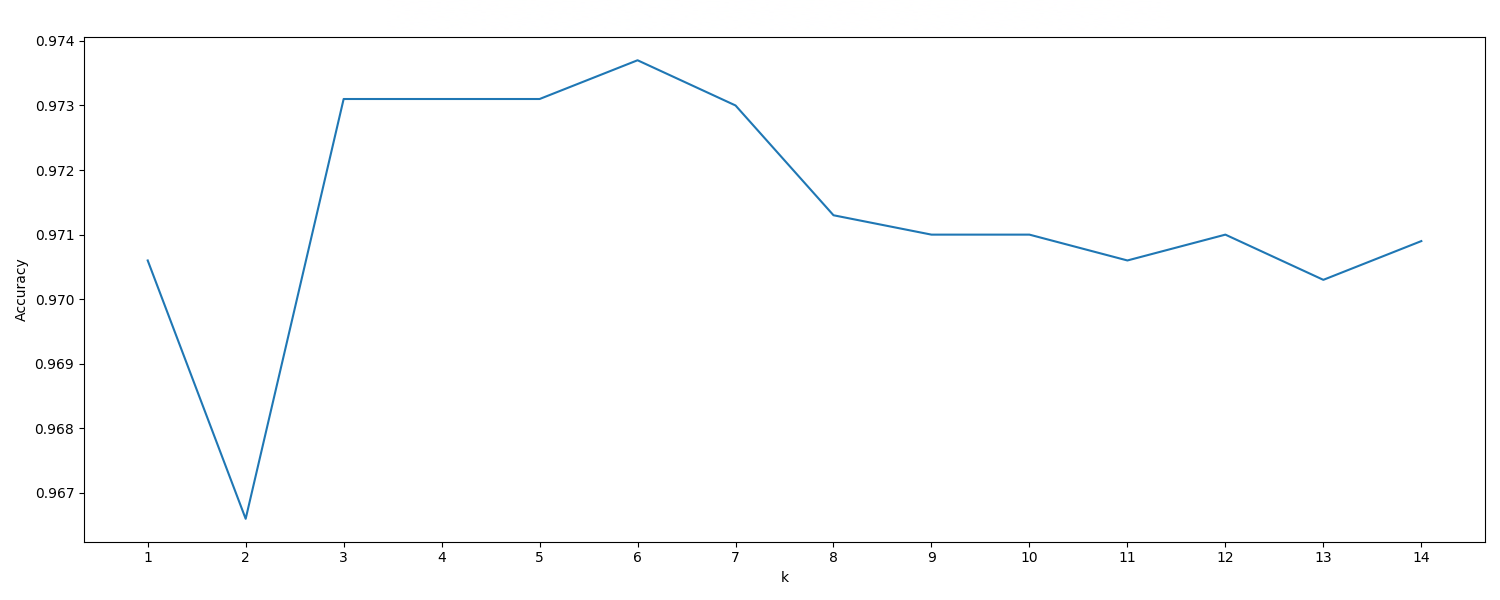
\includegraphics[width=\textwidth]{images/knn.png}
%\caption*{Prediction accuracy of kNN Classifier \\
%as a function of k (Number of Neighbours)}
%\setlength{\belowcaptionskip}{-20pt}
%\setlength{\abovecaptionskip}{-20pt}
%\end{figure}


%\begin{table}[H]
%\centering
%\begin{tabular}{llllllllllll}
%Predicted & 0 & 1     & 2     & 3     & 4    & 5    & 6    & 7     & 8    & 9    & All    \\
%Actual &      &       &       &       &      &      &      &       &      &      &        \\
%0      &  975 &     1 &     1 &     0 &    0 &    1 &    1 &     1 &    0 &    0 &    980 \\
%1      &    0 &  1131 &     1 &     0 &    0 &    0 &    3 &     0 &    0 &    0 &   1135 \\
%2      &    7 &     1 &  1003 &     0 &    1 &    0 &    3 &    11 &    6 &    0 &   1032 \\
%3      &    0 &     2 &     4 &   973 &    0 &   13 &    0 &     6 &   10 &    2 &   1010 \\
%4      &    0 &     0 &     0 &     0 &  960 &    0 &    4 &     2 &    0 &   16 &    982 \\
%5      &    3 &     2 &     1 &     9 &    1 &  868 &    5 &     1 &    1 &    1 &    892 \\
%6      &    4 &     4 &     0 &     0 &    3 &    0 &  947 &     0 &    0 &    0 &    958 \\
%7      &    1 &    20 &    10 &     0 &    2 &    0 &    0 &   985 &    0 &   10 &   1028 \\
%8      &    3 &     0 &     3 &    14 &    4 &    5 &    1 &     2 &  938 &    4 &    974 \\
%9      &    4 &     3 &     3 &    10 &   14 &    6 &    1 &     7 &    4 &  957 &   1009 \\
%All    &  997 &  1164 &  1026 &  1006 &  985 &  893 &  965 &  1015 &  959 &  990 &  10000 \\
%\end{tabular}
%\caption*{Confusion Matrix of kNN classifier with 6 neighbors\\
%Accuracy: 97.37\%}
%\end{table}


%\newpage

\section*{Dictionary Computation}

%At the end of my assignment 1, I was able to find contours in a given sudoku
%image. To use the kNN classifier on each digit on the Sudoku Dataset to get the
%digits, I needed to do some processing. First I did a perspective transform to
%obtain a bird eye view of the sudoku grid. 

%Afterwards, I resized the image to 252 x 252 to iterate over it with 28 by 28
%squares so that I cover a cell with each iteration with a nested loop. In each
%iteration, I cropped 3 pixels from each side of the image and resized the
%cropped image back to 28 x 28.

%\begin{figure}[H]
%\centering
%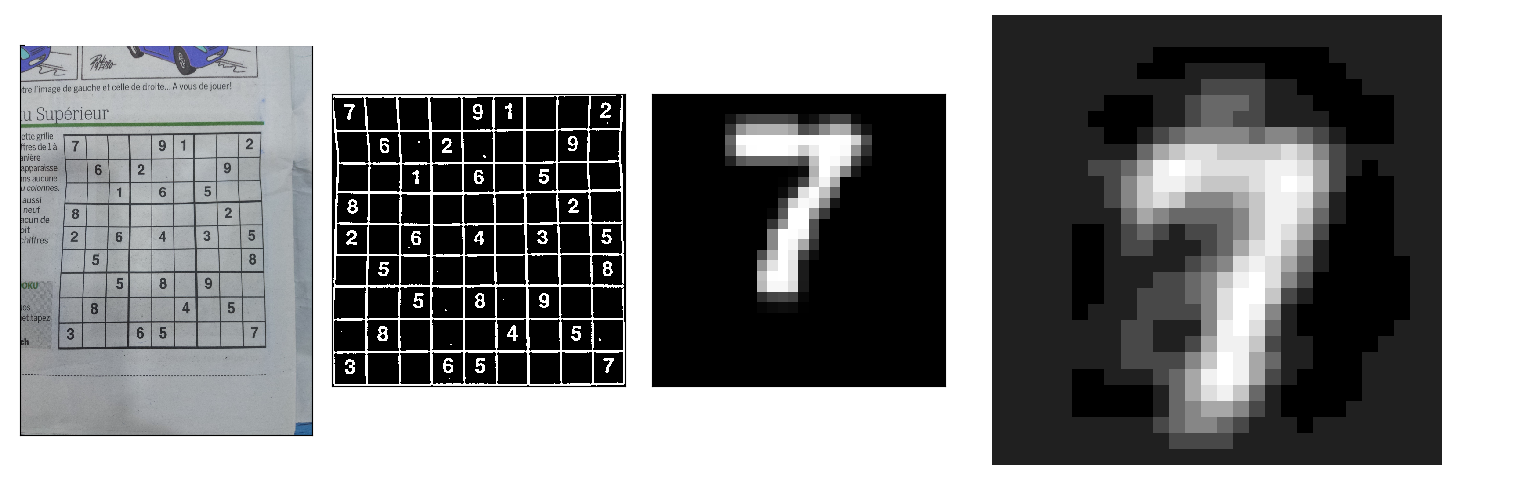
\includegraphics[width=\textwidth]{images/wrapped.png}
%\caption*{Original,wrapped, extracted and Projected Grid}
%\setlength{\belowcaptionskip}{-20pt}
%\setlength{\abovecaptionskip}{-20pt}
%\end{figure}

%After some trial and error, I decided to use the mean of each cell to determine
%if that cell is empty or not. I created a 9 x 9 zero matrix to store the digit
%data, and marked the non empty cells with -1. I projected each extracted cell to
%their first 25 principal components using the principal components I have
%computed at the beginning. I repeated the steps that I have followed for
%computing the distances and predicting the labels this time for the extracted
%pieces from the sudoku grid.

%Lastly I combined the prediction array and the grid array which resulted a final
%9 x 9 array with my predictions and empty cells.


\section*{Feature Quantization and Histogram Calculation}
\section*{Classifier Training}
\section*{Results}

%I can say that the PCA for dimensionality reduction worked really well. In the
%scatter plot, it is easy to see the clustering. The kNN algorithm also did a
%great job in classifying the test images with an accuracy of 97.37\%. For the
%Sudoku predictions, I ended up with 42.11\% accuracy for the sudoku dataset.

%Unfortunately sudoku predictions were not so well because of the problems with
%the extracted image.  They were not looking as clear as the images in the MNIST
%dataset. I believe my algorithm could be improved with better image
%pre-processing. With this project, I had a chance to understand the power of the
%matrix multiplications since they helped me to reduce a process which took 30
%minutes to just a couple of minutes.

